% Request flow of the P01 API (GET /health, GET /hello).
% Build:  tectonic request-flow.tex   ->  request-flow.pdf
\documentclass[tikz,border=12pt]{standalone}
\usepackage[T1]{fontenc}
\usepackage{lmodern}
\usetikzlibrary{positioning,shapes.geometric,arrows.meta,calc,fit}

\definecolor{step}{HTML}{E8F0FE}
\definecolor{stepline}{HTML}{3367D6}
\definecolor{mw}{HTML}{FFF4E0}
\definecolor{mwline}{HTML}{E37400}
\definecolor{ok}{HTML}{E6F4EA}
\definecolor{okline}{HTML}{188038}
\definecolor{err}{HTML}{FCE8E6}
\definecolor{errline}{HTML}{C5221F}
\definecolor{dec}{HTML}{F3E8FD}
\definecolor{decline}{HTML}{8430CE}

\tikzset{
  base/.style={draw, thick, rounded corners=3pt, align=center,
               font=\small, minimum height=11mm, inner sep=5pt},
  box/.style={base, fill=step, draw=stepline, text width=58mm},
  mw/.style={base, fill=mw, draw=mwline, text width=58mm},
  ok/.style={base, fill=ok, draw=okline, text width=58mm},
  err/.style={base, fill=err, draw=errline, text width=50mm},
  dec/.style={diamond, aspect=2.4, draw=decline, fill=dec, thick,
              align=center, font=\small, inner sep=1pt},
  term/.style={base, rounded corners=6mm, fill=white, draw=black,
               text width=40mm},
  arr/.style={-{Stealth[length=2.6mm]}, thick},
  lab/.style={font=\footnotesize\itshape, fill=white, inner sep=1.5pt},
}

\begin{document}
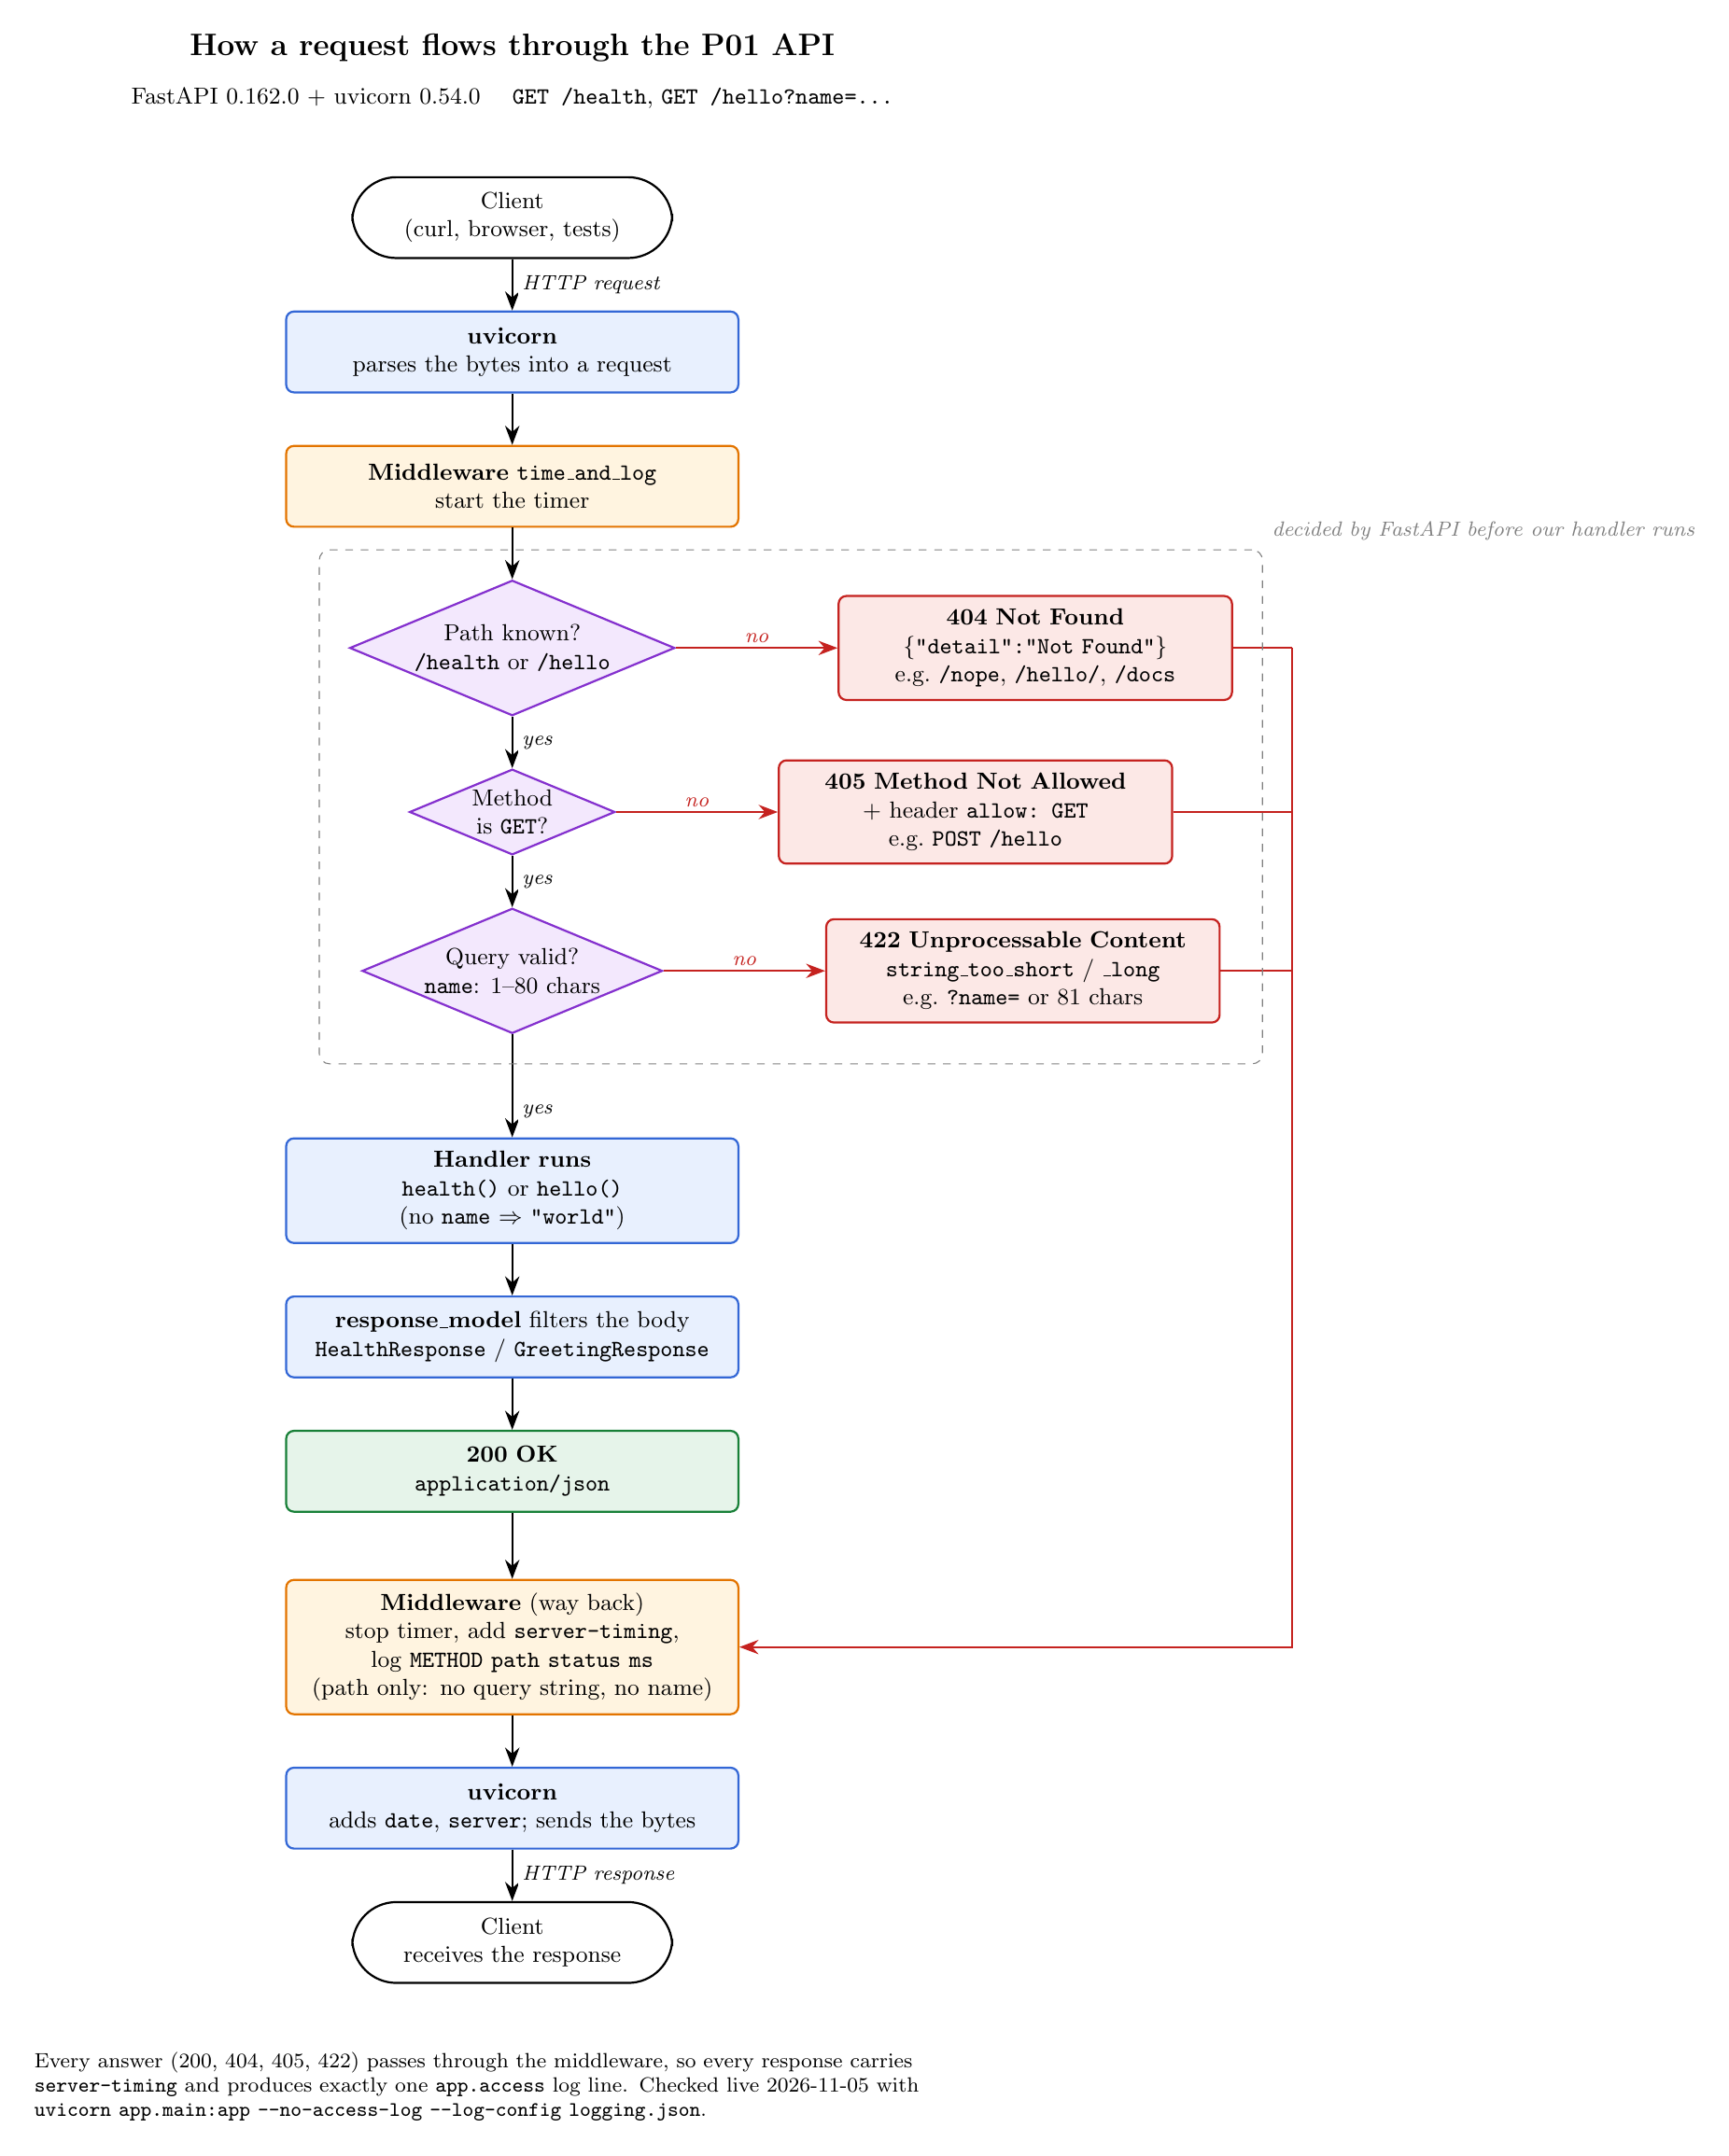
\begin{tikzpicture}[node distance=7mm]

  \node[font=\large\bfseries] (title)
    {How a request flows through the P01 API};
  \node[font=\small, below=1mm of title] (sub)
    {FastAPI 0.162.0 + uvicorn 0.54.0 \quad
     \texttt{GET /health}, \texttt{GET /hello?name=\dots}};

  \node[term, below=8mm of sub] (client) {Client\\(curl, browser, tests)};
  \node[box, below=of client] (uv) {\textbf{uvicorn}\\parses the bytes into a request};
  \node[mw, below=of uv] (mw1) {\textbf{Middleware} \texttt{time\_and\_log}\\start the timer};

  \node[dec, below=of mw1] (path) {Path known?\\\texttt{/health} or \texttt{/hello}};
  \node[dec, below=of path] (meth) {Method\\is \texttt{GET}?};
  \node[dec, below=of meth] (val) {Query valid?\\\texttt{name}: 1--80 chars};

  \node[box, below=14mm of val] (h) {\textbf{Handler runs}\\\texttt{health()} or \texttt{hello()}\\(no \texttt{name} $\Rightarrow$ \texttt{"world"})};
  \node[box, below=of h] (rm) {\textbf{response\_model} filters the body\\\texttt{HealthResponse} / \texttt{GreetingResponse}};
  \node[ok, below=of rm] (ok) {\textbf{200 OK}\\\texttt{application/json}};

  \node[err, right=22mm of path] (e404) {\textbf{404 Not Found}\\\texttt{\{"detail":"Not Found"\}}\\e.g.\ \texttt{/nope}, \texttt{/hello/}, \texttt{/docs}};
  \node[err, right=22mm of meth] (e405) {\textbf{405 Method Not Allowed}\\+ header \texttt{allow: GET}\\e.g.\ \texttt{POST /hello}};
  \node[err, right=22mm of val] (e422) {\textbf{422 Unprocessable Content}\\\texttt{string\_too\_short} / \texttt{\_long}\\e.g.\ \texttt{?name=} or 81 chars};

  \node[mw, below=9mm of ok] (mw2) {\textbf{Middleware} (way back)\\stop timer, add \texttt{server-timing},\\log \texttt{METHOD path status ms}\\(path only: no query string, no name)};
  \node[box, below=of mw2] (uv2) {\textbf{uvicorn}\\adds \texttt{date}, \texttt{server}; sends the bytes};
  \node[term, below=of uv2] (client2) {Client\\receives the response};

  % main path
  \draw[arr] (client) -- node[lab, right=2pt] {HTTP request} (uv);
  \draw[arr] (uv) -- (mw1);
  \draw[arr] (mw1) -- (path);
  \draw[arr] (path) -- node[lab, right=2pt] {yes} (meth);
  \draw[arr] (meth) -- node[lab, right=2pt] {yes} (val);
  \draw[arr] (val) -- node[lab, right=2pt, pos=0.75] {yes} (h);
  \draw[arr] (h) -- (rm);
  \draw[arr] (rm) -- (ok);
  \draw[arr] (ok) -- (mw2);
  \draw[arr] (mw2) -- (uv2);
  \draw[arr] (uv2) -- node[lab, right=2pt] {HTTP response} (client2);

  % error branches
  \draw[arr, errline] (path) -- node[lab, above] {no} (e404);
  \draw[arr, errline] (meth) -- node[lab, above] {no} (e405);
  \draw[arr, errline] (val)  -- node[lab, above] {no} (e422);

  % errors rejoin the middleware on the way back
  \coordinate (rail) at ($(e404.east)+(8mm,0)$);
  \draw[thick, errline] (e404.east) -- (rail);
  \draw[thick, errline] (e405.east) -- (e405.east -| rail);
  \draw[thick, errline] (e422.east) -- (e422.east -| rail);
  \draw[arr, errline] (rail) |- (mw2.east);

  % framework vs our code
  \node[draw=gray, dashed, rounded corners, inner sep=4mm,
        fit=(path)(meth)(val)(e404)(e405)(e422), label={[font=\footnotesize\itshape, gray]north east:decided by FastAPI before our handler runs}] {};

  \node[font=\footnotesize, text width=130mm, align=left, below=8mm of client2] (note)
    {Every answer (200, 404, 405, 422) passes through the middleware, so every
     response carries \texttt{server-timing} and produces exactly one
     \texttt{app.access} log line. Checked live 2026-11-05 with
     \texttt{uvicorn app.main:app -{}-no-access-log -{}-log-config logging.json}.};

\end{tikzpicture}
\end{document}
